%--------------------
% Packages
% -------------------
\documentclass[12pt,a4paper]{article}

\input{my-bib-file/usepackage.tex} 

\usepackage{framed}

\title{ \begin{framed} Quantum Information Theory - 67749 \\ 
Recitation 3, \today \end{framed}  }
%\date{\today}
\date{\vspace{-5ex}}


\addbibresource{my-bib-file/sample.bib} 

\begin{document}

\input{my-bib-file/newcommands.tex} 
%\begin{framed}
\maketitle{ }    
%\end{framed}



\newcommand{\CCZ}{\textbf{CCZ}}
\newcommand{\CCX}{\textbf{CCX}}


\newcounter{enumcirc}
\setcounter{enumcirc}{1} 
\counterwithin{enumcirc}{section}


\newcommand{\advanceday}[1][21]{%
\begingroup
\AdvanceDate[#1]%
\today%
\endgroup
}%


\newcommand{\subqCircEx}[2]{\begin{subfigure}[t]{0.5\textwidth}
        \stepcounter{enumcirc} \caption*{ (\alph{enumcirc}) #1} \centering 
        #2
    \end{subfigure}
}

\newcommand{\qCircEx}[4]{\begin{figure*}[h!]
    \centering
    \subqCircEx{#1}{#2}
    ~ 
    \subqCircEx{#3}{#4}
\end{figure*}
}

\newcommand{\qCircExfullline}[2]{\begin{figure*}[h!]
    \stepcounter{enumcirc} \caption*{ (\alph{enumcirc}) #1}
        \centering 
        #2
\end{figure*}
}

\section{Recitation Overview - Quantum Error Correction Codes.}


In the last lectures, we introduced quantum channels - physical maps between density matrices and mentioned that they are used to represent noise, an error that might occur during either computation or communication. Faults and errors are not unique to the quantum regime and were studied before in the context of (classical) error correction codes and fault tolerance. In this recitation, we are first going to represent what classical error correction codes are, and we will give the Tanner codes as an example of the construction of such codes. Then we will talk about the standard way to model quantum noise, give a basic example of a first quantum code, and then eventually we will give the Toric code.

\newcommand{\cH}{\mathcal{H}}
\newcommand{\ketbra}[1]{\ket{#1}\bra{#1}}
\newcommand{\brakett}[3]{\braket{#1 | #2 | #3}}
\newcommand{\old}[1]{}
\newcommand{\tT}{\tilde{T}}
\newcommand{\trace}{ \mathbf{Tr} }




\part{Classicl Error Correction Code.}

  \section{Codes in General. Notations and Definitions.}
  
A code is a subset, which one can think of as the valid points. Here we focus only on linear binary codes, which are linear subspaces of $\mathbb{F}_{2}^{n}$. As implied at the beginning, codes are used to correct errors, a correctable error is one that gets a valid point into its local environment. A common way to measure resilience is to ask how many bits an evil entity needs to flip such that the corrupted vector will be closer to another vector in that space than the original one. Those ideas were formulated by Hamming \cite{Hamming}, who presented the following definitions. 
  \begin{definition} \label{bi-code} Let $n \in \mathbb{N}$ and $\rho, \delta\in \left( 0,1 \right)$. We say that $C$ is a \textbf{binary linear code} with parameters $[n, \rho n, \delta n]$. If $C$ is a subspace of $\mathbb{F}_{2}^{n}$, and the dimension of $C$ is at least $\rho n$. In addition, we call the vectors belong to $C$ \textit{codewords} and define the distance of $C$ to be the minimal number of different bits between any codewords pair of $C$.   
  \end{definition}
  From now on, we will use the term code to refer to linear binary codes, as we don't deal with any other types of codes. Also, even though it is customary to use the above parameters to analyze codes, we will use their percent forms called the relative distance and the rate of code, matching $\delta$ and $\rho$ correspondingly.     
  \begin{definition} \label{family} A \textbf{family of codes} is an infinite series of codes. Additionally, suppose the rates and relative distances converge into constant values $\rho,\delta$. In that case, we abuse the notation and call that family of codes a code with $[n, \rho n, \delta n]$ for fixed $\rho, \delta\in [ 0,1 )$, and infinite integers $n \in \mathbb{N}$.     
  \end{definition}
  Notice that the above definition contains codes with parameters attending to zero. From a practical view, it means that either we send too many bits, more than a constant amount, on each bit in the original message. Or that for big enough $n$, adversarial, limited to changing only a constant fraction of the bits, could disrupt the transmission. That distinction raises the definition of good codes.

  \begin{definition} \label{good-code} We will say that a family of codes is a \textbf{good code} if its parameters converge into positive values. 
  \end{definition}


  \begin{example}[The Check-sum/Even-parity Code.]
The parity check code $C_{p} \subset \mathbb{F}_{2}^{n+1}$, in which its codewords are only the vectors with even parity.
\begin{equation*}
  \begin{split}
    101 &\mapsto 101 \inb{0} \\ 
    111 & \mapsto 111 \inb{1}\\
    000 & \mapsto 000 \inb{0}
  \end{split}
\end{equation*}
  \end{example}

  \begin{example}[The Repetition Code.]  
    define the repetition code $C_{r} \subset \mathbb{F}_{2}^{n \cdot r}$, In which, for a fixed integer $r$, any bit of the original string is duplicated $r$ times.
\begin{equation*}
  \begin{split}
    0 & \mapsto 0\inb{000}\\
    1 & \mapsto 1\inb{111}
  \end{split}
\end{equation*}
  \end{example}

Having both examples in mind, we get a feeling of the behavior of the distance-rate trade-off. To summarize, using a simple construction, one could construct the codes $[r, 1, r]$ and $[r, r-1, 2]$. Each has a single perfect parameter, while the other decays to the worst. That's bring us to present the Singleton Bound.

  Besides being the first bound, Singleton bound demonstrates how one could get results by using relatively simple elementary arguments. It is also engaging to ask why the proof yields a bound that, empirically, seems far from being tight.
  \begin{theorem*}[Singleton Bound.]\label{theorem*:Sing}  For any linear code with parameter $[n,k,d]$, the following inequality holds:
  \begin{equation*}
    k+ d \le n + 1
  \end{equation*} 
  \end{theorem*}

\begin{proof} Since any two codewords of $C$ differ by at least $d$ coordinates, we know that by ignoring the first $d-1$ coordinate of any vector, we obtain a new code with one-to-one corresponding to the original code. In other words, we have found a new code with the same dimension embedded in $\mathbb{F}_{2}^{n-d+1}$. Combine the fact that dimension is, at most, the dimension of the container space, we get that:  
  \begin{equation*}
    \begin{split}
      \dim C &= 2^{k} \le 2^{n-d+1} \Rightarrow k+d \le n + 1
    \end{split}
  \end{equation*}
\end{proof}

It is also well known that the only binary codes that reach the bound are: $[n,1,n]$, $[n,n-1,2]$,$[n,n,1]$ \cite{eczoo_mds}. In particular, there are no good binary codes that obtain equality(And no binary code which get close to the equality exits). 

Next, we will review Tanner's construction, that in addition to being a critical element to our proof, also serves as an example of how one can construct a code with arbitrary length and positive rate.

\section{Tanner Code}
The constructions require two main ingredients: a graph $\Gamma$, and for simplicity, we will restrict ourselves to a $\Delta$ regular graph, Yet notice that the following could be generalize straightforwardly for graphs with degree at most $\Delta$. The second ingredients is a ;small' code $C_{0}$ at length equals the graph's regularity, namely $C_{0} = [\Delta,\rho\Delta, \delta\Delta]$. We can think about any bit string at length $\Delta$ as an assignment over the edges of the graph. Furthermore, for every vertex $v \in \Gamma$, we will call the bit string, which is set on its edges, the local view of $v$. Then we can define, \cite{Tanner}:
  \begin{definition}  Let $ C = \mathcal{T}\left( \Gamma, C_{0} \right)$  be all the codewords which, for any vertex $v\in \Gamma$, the local view of $v$ is a codeword of $C_{0}$. We say that $C$ is a \textbf{Tanner code}\label{Tan} of $\Gamma, C_{0}$. Notice that if $C_{0}$ is a binary linear code, So $C$ is.  
  \end{definition}
  \begin{example}
Consider the Petersen graph $\Gamma$, which is a regular graph with degree $3$. Let $C_{0}$ be the set of all words with even parity. It follows that $C_{0}$ contains all even-length binary strings of length $3$: $000$, $110$, $101$, and $011$. However, the size of $\mathcal{T}(\Gamma, C_{0})$ is significantly larger, as shown in Figure \cref{fig:pet}. Specifically, any rotation of the inner and outer cycles simultaneously gives rise to another valid codeword, so any assignments that are not invariant under these rotations would produce five additional valid codewords.

  \end{example}

  \begin{figure}[h]
    \centering
    \includegraphics[width=\textwidth]{peterson.png}
    \caption{Peterson Graph.}
    \label{fig:pet}
  \end{figure}


%\end{center}
  %It's also worth mentioning that the first construction of good classical codes, due to Sipser and Shpilman, are Tanner codes over expanders graphs \cite{ExpanderCodes}.
  \begin{lemma}
\label{tanrate} Tanner codes have a rate of at least $2\rho - 1$.
\end{lemma}
  \begin{proof}  The dimension of the subspace is bounded by the dimension of the container minus the number of restrictions. So assuming non-degeneration of the small code restrictions, we have that any vertex count exactly $ \left( 1 - \rho  \right)\Delta $ restrictions. Hence, \begin{equation*}
    \begin{split}
      \dim C & \ge \frac{1}{2}n\Delta - \left( 1-\rho \right)\Delta n = \frac{1}{2}n\Delta\left( 2\rho - 1 \right)  
    \end{split}
  \end{equation*} Clearly, any small code with rate $> \frac{1}{2}$ will yield a code with an asymptotically positive rate \end{proof} 
  %\subsubsection{Positive Rate, Arbitrarily Large Codes.} 
  Based on \cref{tanrate}, we can obtain a recipe for constructing codes with a almost non-vanishing rate for arbitrarily large lengths and dimensions. This recipe involves concatenating a series of Tanner codes over complete graphs. To be more precise, we can define a family of codes as follows:
  \begin{equation*}
    \begin{split}
      C_{i+1} & = \mathcal{T}\left( K_{n(C_{i}) + 1}, C_{i} \right) \\
      C_{0} &= \text{ Some simple } \Delta[1, \rho_{0}, \delta_{0}] \text{ code. }
    \end{split}
  \end{equation*}
Where $n(C_i)$ represents the code length of the $i$th code. Repeating the process described above $\log_{\Delta}^{*}(n)$ times allows us to extend the initial code $\Delta[1,\rho_{0}]$ to $n[1, \sim 2\rho^{\log_{\Delta}^{*}(n)}]$. Interestingly, any family of finite groups generated by a constant-size generator set can define a family of codes by utilizing their Cayley graphs as a basis for Tanner codes.

  Once we have seen that Tanner codes enable us to achieve rates, the next natural question to ask is about the distance of the codes. Achieving a linear distance requires a little bit more from the graphs, but to understand this idea better, let us return to the repetition code. For instance, the repetition code can be presented as a Tanner code over the cycle graph.  

  \begin{example}
    In this representation, each vertex checks if the bits on its edges are equal. A valid codeword is an assignment in which all the bits are equal, since otherwise, there would be an edge with no supporting vertex. An illustration of a legal assignment is provided in \cref{fig:cyc}.
    

Recall that the distance of a linear code is the minimal weight of the non-zero codewords. Consider a codeword $c \in C$ and group the vertices by four sets $V_i$ such that $V_i$ is the set of vertices that see $i \in \{0,1\}^{2}$. Since $c \in C$, we have that $|V_{10}|=|V_{01}| = 0$. Additionally, any vertex in $V_{00}$ is not connected to $V_{11}$, which gives us two possible cases: either all the vertices in $V_{11}$ are isolated, or the graph is not connected. Hence, the distance of the code is equal to $\frac{1}{2}\sum{|V_{i}|\cdot |i|} = \frac{1}{2}2 \cdot n = n$.
  \end{example} 


 \begin{figure}[h]
   \begin{center}
  \label{fig:cyc}
\input{~/workspace/Academic/projects/NLTES_project/ltc_ldpc/network2-cycle.tex} 
\caption{The $1^{n}$ assignment on the cycle graph. Any vertex compute parity $1 + 1 = 0$, therefore all the restrictions are satisfied and $1^n \in \mathcal{T} \left( \text{ cycle } , \text{ parity }  \right) $.}
\end{center}
\end{figure}

It is worth mentioning that, in the literature, the repetition code is not usually given as an example of a Tanner code. However, this example will come up again later in the chapter on quantum codes, when we discuss the Toric code, its relation to the hyperproduct code, and how it can be seen as a hyperproduct of two cycle codes.

Furthermore, analyzing the repetition code gives a clue as to how, in certain cases, one might prove a lower bound on the code distance. We would like to say that, if the weight of the code word is below the distance, then it must be that there is at least one vertex that has a non-trivial local view which is not a codeword in $C_{0}$. Put differently, we cannot spread a small weight codeword over $\{V_{i}\}$, defined above, without expanding into subsets corresponding to low $|i|$. Next, we are going to present the Expander codes, which are Tanner codes constructed from graphs with good algebraic expansion.
%Note that for any $S\subset V$ and $ S \neq V $, 

%But on the other hand any vertex in $V_{00}$ can't be connected to $V_{11}$, Thus we obtain that either all the vertices in $V_{11}$ tr that the graph is not connected. The distance of the code is $\frac{1}{2}\sum{|V_{i}|\cdot |i|} = \frac{1}{2}2 \cdot n = n$.      
% The idea  


\part{Quantum Error Correction Codes.}
\section{Introduction.}
It is widely believed that quantum machines have a significant advantage over classical machines in a wide range of computational tasks \cite{grover1996fast}, \cite{ahuja1999quantum}. Simple algorithms which can be interpreted as the quantum version of scanning all the options, reducing the running time by the square root of the classical magnitude.
Nevertheless, Shor has demonstrated a polynomial-depth quantum circuit that solves the hidden abelian subgroup problem \cite{Shor_1997}, which is considered a breakthrough, as it made the computer science community believe that a quantum computer could offer an exponential advantage.

Despite a consensus on the superiority of the ideal quantum computing model, it is still uncertain whether it is possible to implement such a machine in a noisy environment.
Still, simply pointing out the existence of noise is not sufficient to negate the feasibility of computation. Evidence of this is that classical computers also experience a certain rate of errors. Therefore, to fully comprehend the difficulty, let us compare two main factors that made it a challenging task.


First is the magnitude of the error rate; classical computers also have errors, and sometimes we witness system failures (e.g. the blue screen). The error rate of modern computers is so low that the probability of errors propagating stays negligible, even if the length of the computation is polynomial in the scale of what is considered a reasonable input size. It's worth mentioning that in exascale computing, when supercomputers perform around $10^{18}$ operations per second, it is difficult to overlook faults. In quantum computing, we become aware of their existence much earlier.
 

The second difference, which is a subtle point, is that quantum states are susceptible to additional types of errors. In addition to the possibility of bit-flip errors, a quantum state may also experience a change in phase. For example, consider the initial state $\ket{+} = \frac{1}{\sqrt{2}}\left( \ket{0} + \ket{1} \right)$, and suppose that due to noise the state is transformed into $\frac{1}{\sqrt{4}}\left( \sqrt{3}\ket{0} + \ket{1} \right)$. Classical circuits are oblivious to such faults, meaning that their operation would remain unchanged as no error has occurred. Quantum circuits, however, are usually affected and may fail. Furthermore, when designing a decoder for quantum error correction codes, one must ensure that the decoding process does not introduce bit-flip errors if a classical code is used to protect against phase flips.

\input{~/workspace/Academic/projects/master-thesis/qnoise.tex} 

However, even though quantum noise is so violent, it has been proven that any ideal circuit of polynomial depth can be transformed into a robust circuit at poly-logarithmic cost \cite{aharonov1999faulttolerant}. In other words, there is a threshold: if physicists provide qubits and a finite gate set with a noise rate below that threshold, then BQP, the class of polynomial-time ideal quantum computation, is feasible and can be computed on a realistic machine.


The basic idea in \cite{aharonov1999faulttolerant} was to show the existence of quantum error correction codes, which would enable logic operations to be performed in a way that prevents errors from propagating. This process involves separating the operation into two stages: the operation itself and an error correction stage. This comes with an additional cost in terms of space and time, but it can reduce the probability of the final state being faulty. The trade-off between the resources needed and the rate of decrease defines the threshold. If the balance is positive, then the process can be repeated in a recursive manner, and after log-log iterations, the failure probability will decay to zero. At the same time, the circuit will scale to a maximum of poly-logarithmic width and depth.


Let's return to the repetition code presented in Chapter 2. We would like to have an analog; a first and natural attempt might consider duplicating copies of the state. Unfortunately, copying a general state is not a linear operation and therefore cannot be done in the circuit model (or any other believed to be feasible). In particular, there is no circuit $U$ which can simultaneously duplicate the states $\ket{0}, \ket{1}, \ket{+}, \ket{-}$.

To overcome the issue, Shor came up with the nine-qubit code \cite{Ninequ}, which at first glance might seem a naive straightforward implementation of ``duplication'', but instead uses a clever insight about quantumness in general. Any operation can be seen as a linear (and even unitary) operation over a subspace embedded in a large enough dimension. The encoding is given as follows: 
\begin{equation*}
  \begin{split}
    |\overline{0}\rangle&=\frac{1}{2\sqrt{2}}\left(|000\rangle+|111\rangle\right)^{\otimes3}\\
    |\overline{1}\rangle&=\frac{1}{2\sqrt{2}}\left(|000\rangle-|111\rangle\right)^{\otimes3}~.
  \end{split}
\end{equation*}


For convenience, let us use the notation $\ket{\mathbf{GHZ}^{\pm}} =  \ket{0^{m}} \pm  \ket{1^{m}}$. We can also consider the Shor code over $m^{2}$ qubits, which is defined as above, such that any logical state contains $m$ products over $m$ qubits. Therefore, the state $\ket{\overline{0}}$ over $m^{2}$ qubits can be written as $\ket{\mathbf{GHZ}^{+}}^{m}$. We are now ready to prove a statement regarding the robustness.
\begin{lemma}
  The Shor code over $9$ qubits enable to correct a single either bit or phase flip.  
\end{lemma}
It is evident that a single bit-flip error can be handled in the same way as in the conventional case. The decoder will check if any of the triples have the same value, and if not, it will correct it by majority. To create a decoder that can also correct a phase-flip error, we need the following statement. In this chapter, we denote the Hadamard gate over $m$ qubits as $H^m$.
\begin{claim}
   $H^{m}\ket{\mathbf{GHZ}^{\pm}} = \sum_{ x \cdot \mathbf{1} =_2 \pm }{\ket{x} }$
\end{claim}

\begin{proof}

  \begin{equation*}
    \begin{split}
      H^{m}\ket{\mathbf{GHZ}^{\pm}} & = H^{m}\ket{0^{m}} \pm  H^{m}\ket{1^{m}} = \sum_{x \in \mathbb{F}_{2}^{m}}{\ket{x}} \pm  \sum_{x \in \mathbb{F}_{2}^{m}}{\left( -1 \right)^{x \cdot \mathbf{1}} \ket{x}} \\ & = \sum_{x \in \mathbb{F}_{2}^{m}}{ \left( 1 \pm \left( -1 \right)^{x \cdot \mathbf{1}}  \right) \ket{x} } =  \sum_{x \cdot \mathbf{1} =_2 \pm }{\ket{x} }
    \end{split}
  \end{equation*}
\end{proof}

Now it is clear how to correct a phase flip. One can apply the Hadamard transform and compute the parity of each triple. By the assumption that only a single phase flip may occur, either all the triples have the same parity or the faulted one has an opposite parity and needs to be corrected. Thus, we obtain an $\left[ \left[ 9,1,3 \right] \right]$ quantum error correction code. Asymptotically, this is an $\left[ \left[ m^{2}, 1, m \right] \right]$ code.

\section{CSS Codes.}

The Shor code is a specific case of the more general CSS (Calderbank-Shor-Steane) code \cite{Calderbank_1996}. A family composed by two binary codes $C_{X}, C_{Z}$ such that $C_{Z}^{\perp} \subset C_{X}$. 

\input{~/workspace/Academic/projects/master-thesis/css.tex}

  \section{qLDPC Codes.}
  As exactly as in the classic case, qLDPC codes are codes in which any check act non trivially on at most a constant number of qubits, It was proved that using a good Quantum LDPC code one can achieve a fault tolerance threshold theorem at the cost of only constant overhead\footnote{under the assumption of having an efficient decoder.} \cite{gottesman2014faulttolerant}. We are now about to embark on a detailed review of the first quantum LDPC code \cite{Dennis_2002}. 

  Recall that one way to present a code is by define the parity check matrix, Consider the $l\times l$ Tours, namely the Cayley graph of the group product  $\mathbb{Z}_{l} \times \mathbb{Z}_{l}$. Associate any coordinate (bit/qubit) with an edge on the Tours. And consider the following two restrictions:

  \begin{enumerate}
    \item Each vertex requires form its local view, the bits lay on its supported edges, To has an even party. We will refer to this type of check as \textit{cross check}. 
    \item Similarly, each face requires the same from its supported edges, but computes the parity in a different (specific) base. That it, the face first rotates the qubits by applying the Hadamard transform on them, and then computes their XOR. Finally, the qubits are rotated back to the computation base. We shall refer to this type of check as \textit{face check}.
  \end{enumerate}

  \begin{center}
    \begin{figure}[H]
  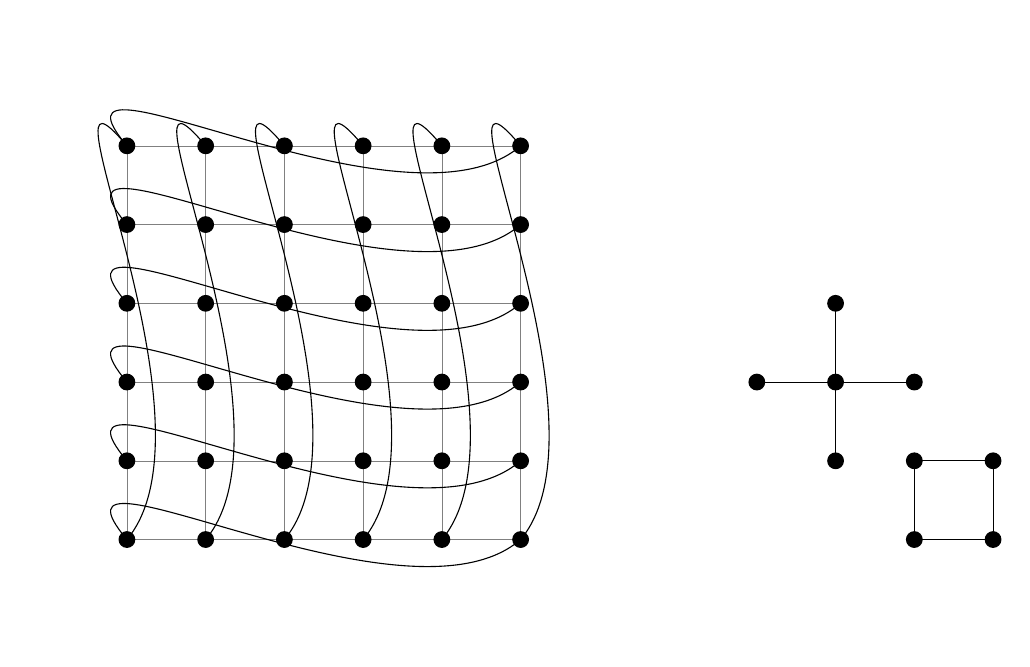
\begin{tikzpicture}
  \draw[step=1cm,gray,very thin] (0,0) grid (5,5);
  \foreach \x in {0,1,2,3,4,5}
  \foreach \y in {0,1,2,3,4,5}
  {
  \node[draw,circle,inner sep=2pt,fill] at (\x,\y) {};
}
\draw[ -> ]  (0,0) to [out=50, in=130] (0,5);
\draw[ -> ]  (1,0) to [out=50, in=130] (1,5);
\draw[ -> ]  (2,0) to [out=50, in=130] (2,5);
\draw[ -> ]  (3,0) to [out=50, in=130] (3,5);
\draw[ -> ]  (4,0) to [out=50, in=130] (4,5);
\draw[ -> ]  (5,0) to [out=50, in=130] (5,5);
\draw[ -> ]  (0,5) to [out=130, in=220] (5,5);
\draw[ -> ]  (0,4) to [out=130, in=220] (5,4);
\draw[ -> ]  (0,3) to [out=130, in=220] (5,3);
\draw[ -> ]  (0,2) to [out=130, in=220] (5,2);
\draw[ -> ]  (0,1) to [out=130, in=220] (5,1);
\draw[ -> ]  (0,0) to [out=130, in=220] (5,0);

\node[draw,circle,inner sep=2pt,fill] at (9,2) {};
\node[draw,circle,inner sep=2pt,fill] at (10,2) {};
\node[draw,circle,inner sep=2pt,fill] at (8,2) {};
\node[draw,circle,inner sep=2pt,fill] at (9,1) {};
\node[draw,circle,inner sep=2pt,fill] at (9,3) {};
\draw[ -> ]  (9,2) to (10,2);
\draw[ -> ]  (9,2) to (8,2);
\draw[ -> ]  (9,2) to (9,1);
\draw[ -> ]  (9,2) to (9,3);
%\draw[ -> ]  (9,2) to (5,0);

\node[draw,circle,inner sep=2pt,fill] at (10,1) {};
\node[draw,circle,inner sep=2pt,fill] at (11,1) {};
\node[draw,circle,inner sep=2pt,fill] at (10,0) {};
\node[draw,circle,inner sep=2pt,fill] at (11,0) {};
\draw[ -> ]  (10,1) to (11,1);
\draw[ -> ]  (10,1) to (10,0);
\draw[ -> ]  (10,0) to (11,0);
\draw[ -> ]  (11,1) to (11,0);
\end{tikzpicture}
\caption{On the left is the Toric Graph. On the right are cross and face checks.}
\label{fig:Toric}
\end{figure}
\end{center}
%For example consider some vertex $v$ on the Torus, and let $\ket{\psi} = \sum_{x}{ \ket{\cdots x_{e_0}x_{e_1}x_{e_2}x_{e_3}  \cdots}}$ when $e_{0},e_{1},e_{2},e_{3}$ are the edges compose the local view of $v$. Then in any ket can be in the support of $\ket{\psi}$ only if the parity of $e_{0},e_{1},e_{2},e_{3}$ is even.
%\subsection{Note on the Toric in the presence of noise.} 

\begin{claim}
  The $l \times l$  Toric code is a CSS code, with dimension $2$ and distance $\Theta\left( l \right)$.   
\end{claim}
\begin{proof}
  Consider a pair of cross and a face checks. If they are not intersect (share edges) then, obviously, they commute. So suppose they share an edge. Now there are a finite number of cases ($4$) in which a cross check can intersect a face, and for all of them we have they must to intersect in an exactly two edges. Therefore the crosses checks commute with all the faces checks. 

  Now, denote by $C_{X}$ and $C_{Z}$ the linear codes defined by the crosses and faces checks. Observes that $C_{X}$ contain all the subgraph of the tours which have only evens degree, namely all the loops. The following claim will be used to show that all the low weight loops (squeezable loops) are in $C_{Z}^{\perp}$. 
  \begin{claim} \label{claim:square}
    Let $c$ be an assignment of ones on a unite square, namely a closed loop at length $4$, then $c \in C_{Z}^{\perp}$.  
  \end{claim}
  \begin{proof}
    Denote by $c^{\prime}$ a codeword of $C_{Z}$, therefore the parity sum induced by $c^{\prime}$ on any square equals zero, Particularly the induced parity on the square supporting $c$ is zero. But that parity is exactly $c\cdot c^{\prime}$. As it true for any $c^{\prime} \in C_{Z}$ we obtain that $c \in C_{Z}^{\perp}$.  
  \end{proof}
  \begin{claim}[Veblen's theorem] \label{claim:velen}
    The set of even subgraph is a linear space spanned by simple cycles (vertices degree equals exactly 2).
  \end{claim}
  \begin{proof}
    Let $P \subset E$ be an even subgraph then it must to have a simple cycle denote it by $P^{\prime}$, now notice that $P/P^\prime$ is also an even subgraph. To see that consider a vertex $v$, As $P^{\prime}$ is simple cycle, substituting $P^{\prime}$ is either not effect the degree of $v$ in $P/P^{\prime}$ or it decrees $v$ degree by exactly $2$ so $d_{P/P^{\prime}}\left( v \right) = d_{P}\left( v \right) - 2$. In both cases $d_{P/P^{\prime}}\left( v \right)$ is even.
    By repeating recursively until $P/P^{\prime} = \{ \emptyset \}$ we get a decomposition of $P$ into a sum of simple cycles.   
  \end{proof}

  \begin{claim}
    \label{claim:inter}
Associate with any vertex of the Torus a coordinate in $\mathbb{Z}_{l} \times \mathbb{Z}_{l}$. Consider a simple cycle $P$ subset of the Torus. Denote $P$ by the vertices composing it $v_{0}v_{1}..v_{k}$ arranged in order. Consider a vertex $v_{i} \in P$  and denote $v = \left( x,y \right) \in $$ \mathbb{Z}_{l} \times \mathbb{Z}_{l}$. Then there exists a vertex $u \in P$, $ u \neq v_{i-1}v_{i+1}$ that shares one of the coordinates of $v$. Put differently, there exists $z$ such that either  $u = \left( z,y \right)$ or $u = \left( x,z \right)$.
  \end{claim}

  \begin{proof} 
Assume without loss of generality that $v_{i-1} = \left( x, y -1 \right)$. Now denote by $f$ the projection on the second coordinate, $f(a,b)= b$. and observe that for any $j$ the distance $f\left( v_{j+1}\right) - \left( v_{j}  \right)$ satisfies:
    \begin{equation*}
      \begin{split}
      f\left( v_{j+1}\right) - f \left( v_{j}  \right) = 
        \begin{cases}
          \pm \left( l - 1 \right)  & v_{j} = \left( \cdot, l -1 \right), v_{j+1} = \left( \cdot, 0  \right)  \\
          \in \{ \pm 1 , 0\} & \text{else}
        \end{cases}
      \end{split}
    \end{equation*}
    So if there is no $u \neq v_{i}$ such that $f(u) = f(v_{i}) = f(v_{i-1})+1$ then there must to be an edge $\{v_{j},v_{j+1}\}$, $v_{j} = \left( \cdot, l -1 \right)$, $ v_{j+1} = \left( \cdot, 0  \right)$ such $P$ pass trough it. So  
    \begin{equation*}
      \begin{split}
        f\left( v_{i-1} \right) & \le f\left( v_{i+1} \right) +  |f\left( v_{i+2} \right) -  f\left( v_{i+1} \right)| + .. + -\left( l - 1 \right) \\ 
        & \le f(v_{i+1}) - |P| - \left(l-1\right)  
      \end{split}
    \end{equation*}
    But $|P| \le l$. 
  \end{proof}
  \begin{figure}[h]
 \begin{tikzpicture}
    \draw [thick, decorate, decoration={random steps,segment length=3pt,amplitude=1pt}]
 (1,0) to[out=90,in=90] (5,0);
    \draw [thick, decorate, decoration={random steps,segment length=3pt,amplitude=1pt}]
 (5,0) to[out=270,in=270] (1,-0.3);
 \filldraw[black] (1,0) circle (2pt) node[anchor=west]{$v_{i+1}$};
 \filldraw[black] (1,-0.3) circle (2pt) node[anchor=west]{$v_{i}$};
 \filldraw[black] (5,0) circle (2pt) node[anchor=west]{$u$};
\draw[draw=gray] (0,-3) rectangle ++(7,7);

\draw [thick, decorate, decoration={random steps,segment length=3pt,amplitude=1pt}]
 (9,0) to[out=90,in=270] (11,4);
    \draw [thick, decorate, decoration={random steps,segment length=3pt,amplitude=1pt}]
 (11,-3) to[out=90,in=270] (9,-0.3);
 \filldraw[black] (9,0) circle (2pt) node[anchor=west]{$v_{i+1}$};
 \filldraw[black] (9,-0.3) circle (2pt) node[anchor=west]{$v_{i}$};
 %\filldraw[black] (13,0) circle (2pt) node[anchor=west]{$u$};
\draw[draw=gray] (8,-3) rectangle ++(7,7);


    %\draw [thick, decorate, decoration={random steps,segment length=10pt,amplitude=2pt}]
 %(0,0) to[out=0,in=0] (0,4);
  \end{tikzpicture}
\caption{
A simple cycle $P$ that passes through a vertex $u$, with the same $y$-coordinate as $v_i$, on the left versus a cycle path for which there is no such $u$.
}
\end{figure}

  \begin{definition}
    Horizontal and Vertical diameters. Let $P$ be defined again as exactly as in \cref{claim:inter}. We will say that the \textit{horizontal diameter} of $P$ is: 
    \begin{equation*}
      \begin{split}
        \max_{v,u\in P} \min{ \left\{  | v_{x} -u_{x}|, |v_{x} + l + u_{x}| \right\} }  
      \end{split}
    \end{equation*}
    Similarly, we define the vertical diametr to be: 
    \begin{equation*}
      \begin{split}
        \max_{v,u\in P} \min{ \left\{  | v_{y} -u_{y}|, |v_{y} + l + u_{y}| \right\} }  
      \end{split}
    \end{equation*}
  \end{definition}

  \begin{claim} \label{claim:reduce}
If $P$ is a non empty simple cycle with vertical and horizontal diameters $d_{1}, d_{2}$, then it can either be a square or can be decomposed into two simple cycles $P_{1},P_{2}$ with either the vertical diameter of both of them being strictly less than $d_{1}$ and their horizontal diameters being at most $d_{2}$, or the horizontal diameter of both of them being strictly less than $d_{2}$ and their vertical diameters being at most $d_{1}$.
  \end{claim}

  \begin{proof} 
%    Assuming $P$ is not a square, it must have either a vertical or horizontal diameter greater than $1$. Let us assume, without loss of generality, that the vertical diameter is greater than $1$. Denote by $v_{0}v_{1}..v_{k}$ the vertices compose $P$, and assume that $v_{i},v_{j}$ are the vertices at maximal distace. Now Pick the first vertex $v_{i^\prime}$ form left to $v_{i}$ such that $v_{i^\prime , y} \neq v_{i,y}$. By \cref{claim:inter} there is at least one vertex $v_{l}$ in $P$ such that $v_{i,y} = v_{l,y}$ takes the one who closet in horizontal distance to $v_{i}$. Now denote by $P^{\uparrow}$ the path $v_{i},v_{i+1}..v_{l-1},v_{l}$ and by $P^{\downarrow}$ the path $v_{l},v_{l+1}..v_{i-1},v_{i}$. Denote by $L$ the stright line $v_{i},\left( v_{i,x}+1, v_{i,y} \right), \left( v_{i,x}+2, v_{i,y} \right), .. v_{l}$. 
%    Assume that both $P^{\uparrow}\cup L$,$P^{\downarrow}\cup L$ are simple cycles, Clearly the vertical diameter is lower by exectly $1$ than the vertical diameter of $P$, also the horizontal distance between any point on $L$ to other point on $P$ is lower than the horizontal distance of between the end of $L$ (namely $\{v_{i},v_{l}\}$), to the same point. Therfore In that case we have the claim.   
%    So it's left to show that $P^{\uparrow}\cup L$,$P^{\downarrow}\cup L$ must to be a simple cycles. Suppose that $P^{\uparrow}\cup L$ is not a simple cycle. So the path $v_{i},v_{i+1}..v_{l-1},v_{l}.. \left( v_{i,x}+2, v_{i,y} \right), \left( v_{i,x}+1, v_{i,y} \right)v_{i}$  must to contain an inner loop. Obivesly the loop can't be supported on $P^{\uparrow}$ alone, because $P^{\uparrow} \subset P$ so the inner loop would has to be contained also in $P$ in controdiction for $P$ be a simple cycle. Thefore, the inner loop is also supported on $L$, So it follows that there is an vertex in $L$ a vertex with degree $>2$ in $P^{\uparrow}\cup L$, namely a vetex $u \neq v_{i},v_{l}$ such that $u_{y} = v_{i,y}$, and also $u \in P$. But by the construction of $L$, $|u_{x} - v_{i,x}| < |v_{l,x} - v_{i,x}|$ in contradiction to the fact that $v_{l}$ chosen to miniazie an horizontal distance.  
%
If $P$ is not a square, it must have either a vertical or horizontal diameter greater than $1$. We will assume, without loss of generality, that the vertical diameter is greater than $1$. Let $v_{0}v_{1}..v_{k}$ be the vertices that compose $P$, and let $v_{i},v_{j}$ be the vertices at maximal distance. We will pick the first vertex $v_{i^\prime}$ from the left of $v_{i}$ such that $v_{i^\prime , y} \neq v_{i,y}$. By \cref{claim:inter}, there must be at least one vertex $v_{l}$ in $P$ such that $v_{i,y} = v_{l,y}$ and is the closest in horizontal distance to $v_{i}$. We will denote by $P^{\uparrow}$ the path $v_{i},v_{i+1}..v_{l-1},v_{l}$ and by $P^{\downarrow}$ the path $v_{l},v_{l+1}..v_{i-1},v_{i}$. We will also denote by $L$ the straight line $v_{i},\left( v_{i,x}+1, v_{i,y} \right), \left( v_{i,x}+2, v_{i,y} \right), .. v_{l}$. 

Observes that the vertical diameter will be lower by exactly $1$ than the vertical diameter of $P$, and the horizontal distance between any point on $L$ to other point on $P$ will be lower than the horizontal distance of between the end of $L$ (namely $\{v_{i},v_{l}\}$), to the same point. So if $P^{\uparrow}\cup L$,$P^{\downarrow}\cup L$ are simple cycles then we get the desire. 
Suppose that $P^{\uparrow}\cup L$ is not a simple cycle. This means that the path $v_{i},v_{i+1}..v_{l-1},v_{l}.. \left( v_{i,x}+2, v_{i,y} \right), \left( v_{i,x}+1, v_{i,y} \right)v_{i}$ must contain an inner loop. This loop cannot be supported on $P^{\uparrow}$ alone, because $P^{\uparrow} \subset P$ so the inner loop would have to be contained also in $P$, which is a contradiction. Therefore, the inner loop is also supported on $L$, so it follows that there is a vertex in $L$ with degree $>2$ in $P^{\uparrow}\cup L$, namely a vetex $u \neq v_{i},v_{l}$ such that $u_{y} = v_{i,y}$, and also $u \in P$. But by the construction of $L$, $|u_{x} - v_{i,x}| < |v_{l,x} - v_{i,x}|$, which is a contradiction to the fact that $v_{l}$ was chosen to minimize the horizontal distance. Thus, we have our claim.
  \end{proof}

%  Now we are ready to proof the claim. Let $c\in C_{X}$ such that $|c| < l$. By \cref{claim:velen}, $c$ decompise into simple cycles. Any of them at weight less than $l$. By applaying $\cref{claim:reduce}$ we have that any of them can decompise into sum of unite squres. But, by \cref{claim:square}, unit squres are in $C_{Z}^{\perp}$ and therfore $c \in C^{\perp}$. 

We have now established that $c \in C_{X}$ with $|c| < l$ can be decomposed into simple cycles, each of which has a weight less than $l$. Applying \cref{claim:reduce} recursively, we can further decompose each of these cycles into a sum of unit squares. However, \cref{claim:square} states that unit squares are in $C_{Z}^{\perp}$, so $c \in C^{\perp}$.
    \begin{wrapfigure}{R}{2cm}
%\begin{tikzpicture}
%    \draw [thick, decorate, decoration={random steps,segment length=3pt,amplitude=1pt}]
% (1,0) to[out=90,in=90] (3,0);
%    \draw [thick, decorate, decoration={random steps,segment length=3pt,amplitude=1pt}]
% (3,0) to[out=270,in=270] (1,0);
% \filldraw[black] (1,0) circle (2pt) node[anchor=east]{$v$};
% \filldraw[black] (3,0) circle (2pt) node[anchor=west]{$u$};
%\draw (1,0) -- (3,0);
%  \end{tikzpicture}
\end{wrapfigure}
%If $P$ is a non empty simple cycle with vertical and horizontal diameters $d_{1}, d_{2}$, then it can either be a square or can be decomposed into two simple cycles $P_{1},P_{2}$ with either the vertical diameter of both of them being strictly less than $d_{1}$ and their horizontal diameters being at most $d_{2}$, or the horizontal diameter of both of them being strictly less than $d_{2}$ and their vertical diameters being at most $d_{1}$.
%
  %\end{proof}

%  \begin{claim}
%  Any Simple cycle can be decmopise as sum of unite squares.     
%  \end{claim}
%
%  Let $c \in C_{X}$ at weight at most $l$ and by $G = (V,E)$ the Cayley graph of the tours, we will refer to each of the two generators of $G$ as directions. We will say that a tuple of edges $\{e_{1},e_{2}\}$ is corner of $c$ if they are both non zero coordinates of $c$ and in addition they match to different directions\footnote{On planner drawing, corner is just an horizontal edge followed by vertical edge}.        
% 
\end{proof}
Note that the subtraction of any two $l$-length vertical cycles is a code word of $C_Z'$ (one can be obtained by adding unit rectangles to the other). Therefore, we have only two non-trivial cosets in $C_X/C_Z'$. Hence, the dimension of the code is two. 

%The Toric code is a topological quantum error-correcting code that encodes a single qubit of information into a two-dimensional lattice of qubits. It is a stabilizer code, meaning that it uses a set of commuting operators to detect and correct errors. The code is based on the mathematical structure of a torus, and its properties make it a powerful tool for quantum computing. It is also a fault-tolerant code, meaning that it can correct errors even when some of the qubits are faulty.
%
%\begin{center}
%  \begin{tikzpicture}
%    \input{shor_decoder.tikz}
%  \end{tikzpicture}
%\end{center}

%\begin{algorithm}[H]
%  \caption{Shor code decoder.}
%    \label{alg:shordecoder}
%    \KwData{ $ \ket{\psi} \in \mathbb{C}_{2}^{9}$ }
%    \KwResult{ Correct a single fault. }
%    Let $D$ be a decoder for the classic repetition code over $3$ qubits. \\ 
%    Let $\ket{x_{1}x_{2}x_{3}} \leftarrow \ket{\psi}$ \\ 
%
%    $ L \leftarrow \text{Array} \{ \} $\\
%    \For { $ v \in V$} {
%      $c^{\prime}_{v} \leftarrow \arg\min {\left\{  y \in C_{0} : |y + x|_{v} |  \right\} } $\\
%      $ L_{v} \leftarrow c^{\prime}_{v}$
%    }
%    $ z \leftarrow \sum_{v \in V}{c^{\prime}_{v}} $\\
%    \eIf{ $ |z| < \tau \frac{n}{f\left( n \right)} $}{
%      \While{ $|z| > 0$ }{
%	find $v$ and $c \in C_{0}$ such that $|z + c_{v}| < |z|$\\
%	$z \leftarrow z + c_{v}$ \\
%	$ L_{v} \leftarrow  L_{v} + c_{v}$
%      }
%    }{
%      reject. 
%    }
%    \Return  $S(L) $
%
%  \end{algorithm}

%
%By quadric the dimension of the repetition code one can find those state which at least two pauli are needed to applay for flipping either the bit or the phase of the logic state. Clearly any phase flip 
 





\printbibliography 


\end{document}

